% =====================================================================
%  PALET — Auditoría técnica y metodológica + plan de mejora
%  Destinatarios: R. Martínez de Vega Perancho, F. Rubiera Morollón
%                 y el agente implementador (Claude Fable 5.2)
%  Compilar: pdflatex x2 (o latexmk -pdf)
% =====================================================================
\PassOptionsToPackage{obeyspaces,spaces}{url}
\documentclass[11pt,a4paper]{article}

\usepackage[T1]{fontenc}
\usepackage[utf8]{inputenc}
\usepackage{lmodern}
\usepackage{babel}
\babelprovide[main,import]{spanish}
\usepackage[margin=2.3cm]{geometry}
\usepackage{microtype}
\usepackage{booktabs,longtable,tabularx,array,multirow}
\usepackage[table]{xcolor}
\usepackage{enumitem}
\usepackage{listings}
\usepackage[most]{tcolorbox}
\usepackage{tikz}
\usetikzlibrary{arrows.meta,positioning,shapes.geometric}
\usepackage{fancyhdr}
\usepackage[hidelinks]{hyperref}

% ---------- Colores y macros ----------
\definecolor{palet}{HTML}{0F766E}
\definecolor{crit}{HTML}{B91C1C}
\definecolor{alto}{HTML}{C2410C}
\definecolor{medio}{HTML}{A16207}
\definecolor{bajo}{HTML}{4B5563}
\definecolor{codebg}{HTML}{F5F7F8}

\newcommand{\sevC}{\textcolor{crit}{\textbf{[C]}}}
\newcommand{\sevA}{\textcolor{alto}{\textbf{[A]}}}
\newcommand{\sevM}{\textcolor{medio}{\textbf{[M]}}}
\newcommand{\sevB}{\textcolor{bajo}{\textbf{[B]}}}
\usepackage{url}
\DeclareUrlCommand\file{\urlstyle{tt}}
\DeclareUrlCommand\code{\urlstyle{tt}}
\newcommand{\WP}[1]{\textbf{\textcolor{palet}{WP#1}}}

\newtcolorbox{nota}[1][]{colback=palet!5,colframe=palet,fonttitle=\bfseries,title=#1,boxrule=0.6pt,arc=2pt}
\newtcolorbox{alerta}[1][]{colback=crit!4,colframe=crit,fonttitle=\bfseries,title=#1,boxrule=0.6pt,arc=2pt}
\newtcolorbox{agente}[1][]{colback=blue!3,colframe=blue!50!black,fonttitle=\bfseries,title=#1,boxrule=0.6pt,arc=2pt}

\lstset{
  basicstyle=\ttfamily\footnotesize,
  backgroundcolor=\color{codebg},
  frame=single, rulecolor=\color{gray!40},
  breaklines=true, columns=fullflexible, keepspaces=true,
  showstringspaces=false, tabsize=2,
  keywordstyle=\color{palet}\bfseries,
  commentstyle=\color{gray}\itshape
}

\setlist{itemsep=2pt,topsep=3pt}
\setlength{\parskip}{4pt}
\setlength{\parindent}{0pt}
\renewcommand{\arraystretch}{1.2}

\pagestyle{fancy}
\fancyhf{}
\lhead{\small PALET — Auditoría y plan de mejora}
\rhead{\small 11 de noviembre de 2026}
\cfoot{\small\thepage}

\begin{document}

% =====================================================================
\begin{titlepage}
\centering
\vspace*{2cm}
{\color{palet}\rule{\linewidth}{1.2pt}}\\[0.6cm]
{\LARGE\bfseries PALET: auditoría técnica y metodológica\\[0.2cm] y plan de mejora}\\[0.4cm]
{\large Del ``buscador + clasificador'' actual a una herramienta de revisión de alcance asistida por IA defendible ante cualquier \emph{referee}}\\[0.4cm]
{\color{palet}\rule{\linewidth}{1.2pt}}\\[1.2cm]

\begin{tabularx}{\linewidth}{rX}
\textbf{Proyecto:} & PALET (Prompt-based Automated Literature Extraction Tool), ISABEL — GA 101177687\\
\textbf{Base revisada:} & carpeta \file{palet/} (commit \code{da90731}), corpus del capítulo y los dos informes de \emph{referees} (\file{ISABELCHAPTER REV.docx})\\
\textbf{Fecha:} & 11 de noviembre de 2026\\
\textbf{Destinatarios:} & Ricardo Martínez de Vega Perancho, Fernando Rubiera Morollón y el agente implementador (Claude Fable 5.2)\\
\end{tabularx}

\vfill
\begin{agente}[Nota para el agente implementador]
Este documento es a la vez un diagnóstico y una especificación. Lee primero el Resumen ejecutivo (§\ref{sec:resumen}) y las Instrucciones operativas (§\ref{sec:instrucciones}). Después ejecuta los paquetes de trabajo de §\ref{sec:wps} \emph{en el orden indicado}, uno a uno, cumpliendo sus criterios de aceptación antes de pasar al siguiente. Cada afirmación sobre el código remite a un fichero; verifícala antes de cambiar nada.
\end{agente}
\end{titlepage}

\tableofcontents
\newpage

% =====================================================================
\section{Resumen ejecutivo}\label{sec:resumen}

\subsection*{Veredicto}

La idea de PALET es buena y la base de ingeniería es razonable para un primer prototipo: fases con nombre, artefactos JSON por fase, \emph{prompts} cuidados y una GUI usable. Pero los dos \emph{referees} han dado en el clavo, y el problema no es cosmético sino \textbf{estructural}. Hoy PALET es, en esencia, \textbf{un buscador seguido de un clasificador temático}; \textbf{no es todavía un \emph{pipeline} de revisión de alcance}. En concreto:

\begin{enumerate}
  \item \textbf{No criba con criterios de elegibilidad.} El LLM decide si un \emph{abstract} ``responde a alguna RQ'', pero los criterios de inclusión/exclusión que genera ARQ nunca se aplican. Por eso entran estudios sobre China, Perú o pérdidas de fósforo.
  \item \textbf{No deja rastro auditable.} No hay razones de exclusión, la cadena de búsqueda real no se archivó, la fecha de búsqueda no se registra y los errores del modelo se cuentan como exclusiones.
  \item \textbf{No mide su propia fiabilidad.} No hay comparación con cribado humano, ni recall de la búsqueda, ni estabilidad entre ejecuciones. Afirmar que el procedimiento es ``objetivo'' o que hace un ``barrido completo'' no se sostiene, y los \emph{referees} lo han visto.
  \item \textbf{La síntesis no está anclada a las fuentes.} No exige citas por afirmación ni comprueba que la fuente diga lo que se le atribuye: es exactamente el fallo M4/M5 del Referee~2.
  \item \textbf{La búsqueda no está diseñada para RQs heterogéneas.} Se usa una sola cadena booleana para todas las RQs (en OpenAlex, que además busca en el texto completo), se trunca en silencio a los primeros $N$ resultados por relevancia y no se guarda el número total de resultados encontrados.
\end{enumerate}

\begin{nota}[Matiz importante sobre el capítulo]
Los 142 artículos del capítulo \textbf{no salieron del código Python actual}. Salieron del flujo de primavera de 2025: una exportación CSV de Scopus con 235 registros (\file{Prueba Final/Final_Fernando_3.1.csv}), clasificada en Excel como \emph{Admitido/No admitido} con una RQ por artículo (\file{Prueba_Final_clasificado.xlsx}). El código se escribió después para replicar ese proceso (el meta-prompt fija como objetivo ``\textasciitilde142 papers''). Aun así, \textbf{el código actual reproduciría los mismos fallos}, y añade otros (§\ref{sec:debilidades}). Las dos cosas hay que arreglarlas a la vez: la herramienta y la forma de contarla en el capítulo.
\end{nota}

\subsection*{Evidencia cuantitativa (corpus del capítulo)}

\begin{itemize}
  \item 235 registros de Scopus $\to$ 234 en la hoja de clasificación: \textbf{un registro desapareció sin rastro} (``Why levelling-up is unlikely to solve regional disparities'', 2020, sin autores en la exportación).
  \item 142 incluidos / 92 excluidos, \textbf{sin ninguna razón de exclusión registrada}.
  \item Un cribado heurístico por palabras clave (título, resumen y palabras clave del autor) da lo siguiente. De los 142 incluidos, \textbf{40 (28\%) no mencionan Europa, la UE ni ningún Estado miembro}, y \textbf{22} mencionan explícitamente solo contextos no europeos. Además, \textbf{65 (46\%) no contienen ningún término de mercado laboral} (\emph{employ*, job*, labo(u)r, work*, skill*}) en título ni resumen.
  \item Hay \textbf{un duplicado no detectado}: Coaquira et al.\ (2022, sin DOI) y Velásquez et al.\ (2023, \code{10.13043/DYS.94.4}) son el mismo trabajo sobre Perú, con título bilingüe y fechas distintas. La deduplicación por DOI exacto o título exacto no puede detectarlo.
  \item La distribución está muy desequilibrada: RQ3 = 61, RQ6 = 39, RQ1 = 18, RQ2 = 13, RQ7 = 5, RQ4 = 4, RQ5 = 2. Cada artículo tiene una sola RQ, pese a que el texto del capítulo sugiere una asignación múltiple.
\end{itemize}

\subsection*{Puntuación actual y objetivo}

\begin{center}
\begin{tabular}{lccl}
\toprule
\textbf{Dimensión} & \textbf{Hoy} & \textbf{Objetivo} & \textbf{WPs clave}\\
\midrule
Ingeniería de software (estructura, robustez, tests) & 5/10 & 9/10 & 0, 1, 11\\
Diseño y ejecución de la búsqueda & 3/10 & 9/10 & 3, 4\\
Cribado / elegibilidad & 2/10 & 9/10 & 5, 7\\
Validación y fiabilidad medida & 0/10 & 9/10 & 6\\
Trazabilidad y reproducibilidad & 3/10 & 10/10 & 1, 9\\
Síntesis anclada a evidencia & 3/10 & 9/10 & 8\\
Cumplimiento PRISMA-ScR / RAISE & 2/10 & 9/10 & 9\\
Usabilidad (GUI, humano en el bucle) & 6/10 & 9/10 & 2, 5, 11\\
\midrule
\textbf{Global (como método publicable)} & \textbf{$\approx$3/10} & \textbf{9--10/10} & \\
\bottomrule
\end{tabular}
\end{center}

\subsection*{Los 10 cambios que más mueven la aguja}

\begin{enumerate}
  \item \textbf{Protocolo primero y congelado} (\WP{2}): las RQs son del investigador, no del LLM. Criterios PCC (población, concepto, contexto) explícitos y aprobados por humanos.
  \item \textbf{Nueva fase SCREEN} (\WP{5}): decisión por criterio, con cita textual del resumen, código de razón de exclusión y categoría \emph{unclear} que va a revisión humana.
  \item \textbf{Dos cribadores independientes más adjudicación humana} de discrepancias e \emph{unclear} (\WP{5}).
  \item \textbf{Fase VALIDATE} (\WP{6}): muestra estratificada cribada por dos humanos a ciegas, con sensibilidad, especificidad, precisión y $\kappa$ con IC del 95\%, más recall de la búsqueda frente a un conjunto de referencias conocidas.
  \item \textbf{Búsqueda por bloques conceptuales y por RQ} (\WP{3}), con OpenAlex restringido a título y resumen (\code{search.title_and_abstract}) y \textbf{API key}, adaptador de Scopus y registro del recuento total y de la fecha de búsqueda.
  \item \textbf{Deduplicación difusa} por DOI, título normalizado, primer autor y año (\WP{4}).
  \item \textbf{Errores $\neq$ exclusiones} (\WP{0}, \WP{5}): todo registro tiene un estado y una razón.
  \item \textbf{Extracción estructurada más síntesis con citas verificadas automáticamente} (\WP{8}): cada afirmación lleva IDs de artículos y una cita literal que se comprueba contra la fuente.
  \item \textbf{Informe PRISMA completo} (\WP{9}): diagrama PRISMA 2020 con razones, \emph{checklist} PRISMA-ScR de 22 ítems, apéndice de métodos reproducible y declaración de uso de IA conforme a RAISE.
  \item \textbf{Manifiesto de ejecución y caché} (\WP{1}): hash del código, IDs exactos de modelo, \emph{hashes} de los \emph{prompts}, parámetros, respuestas crudas de las API y de los LLM. Así una re-ejecución reproduce exactamente las decisiones.
\end{enumerate}

% =====================================================================
\section{Alcance y fuentes revisadas}

\begin{itemize}
  \item \textbf{Código}: \file{palet.py}, \file{app.py}, \file{prisma_validator.py}, \file{scripts/arq_module.py}, \file{scripts/qsp_module.py}, \file{scripts/se_module.py}, \file{scripts/map_module_v2.py}, \file{scripts/synthesis_module.py}, \file{scripts/report_generator_v2.py} (lectura parcial dirigida) y \file{scripts/export_bibtex.py}. Además, los \emph{prompts} \file{arq_system_v3.txt}, \file{qsp_system_v2.txt}, \file{map_system_v2.txt} y \file{synthesis_system.txt}, \file{requirements.txt}, \file{.gitignore} y \file{README.md}.
  \item \textbf{Ejecuciones}: \file{runs_history.json} y salidas en \file{outputs/json/} (ARQ, QSP, MAP; febrero--junio de 2026).
  \item \textbf{Corpus del capítulo}: \file{Prueba Final/} (CSV Scopus, Excel de clasificación y tabla \file{pi_reference_table.tex}).
  \item \textbf{Documentos}: informes de los dos \emph{referees} y borrador de respuesta (\file{ISABELCHAPTER REV.docx}), D2.3 de ISABEL y meta-prompt del agente.
  \item \textbf{Fuentes externas}: documentación vigente de OpenAlex y de la Scopus API, declaración conjunta Cochrane/Campbell/JBI/CEE sobre IA (RAISE) y literatura sobre cribado con LLM (§\ref{sec:refs}).
\end{itemize}

\textbf{No revisado}: \file{palet_codex/} (copia anterior; parece un \emph{fork} de marzo de 2026), \file{static/} y \file{templates/} en detalle, y las líneas 600--1334 de \file{report_generator_v2.py} salvo los puntos citados. La copia conectada como \file{Revision Bibliografia con Fernando/palet} estaba vacía; \textbf{la copia de trabajo real es} \texttt{Artículo Revision Bibliografia con Fernando/palet/}.

% =====================================================================
\section{Diagnóstico empírico del corpus del capítulo}\label{sec:diagnostico}

\subsection{Cribado heurístico por RQ}

El cálculo se hizo sobre \file{Prueba_Final_clasificado.xlsx}. ``Menciona UE'' significa que título, resumen o palabras clave contienen Europa/UE, un Estado miembro, el Reino Unido, \emph{cohesion policy}, \emph{smart specialisation} o NUTS. ``Término laboral'' significa \emph{employ*, job*, labo(u)r, work*, skill*} o \emph{unemploy*} en título o resumen. Es un indicador grueso, no un cribado: sirve para dimensionar el problema, no para decidir inclusiones.

\begin{center}
\begin{tabular}{lrrrl}
\toprule
\textbf{RQ} & \textbf{n} & \textbf{\% menciona UE} & \textbf{\% término laboral} & \textbf{Lectura}\\
\midrule
RQ1 (transición verde) & 18 & 78 & 100 & razonable\\
RQ2 (digital/IA) & 13 & 85 & 77 & razonable\\
RQ3 (cohesión / S3) & 61 & 74 & 38 & \textcolor{crit}{cajón de sastre}\\
RQ4 (educación) & 4 & 100 & 100 & \textcolor{crit}{muy escaso y mal asignado}\\
RQ5 (inmigración) & 2 & 50 & 100 & \textcolor{crit}{muy escaso; 1 sobre China}\\
RQ6 (transición justa) & 39 & 56 & 49 & \textcolor{alto}{mucho no-UE}\\
RQ7 (lagunas de medición) & 5 & 100 & 20 & \textcolor{alto}{poco laboral}\\
\midrule
Total & 142 & 72 & 54 & \\
\bottomrule
\end{tabular}
\end{center}

\subsection{Hallazgos}

\begin{enumerate}
  \item \textbf{RQ3 actuó como sumidero.} Tal como está redactada (``What cohesion or smart-specialisation policies does the evidence suggest?''), no lleva ancla geográfica ni laboral. Cualquier trabajo de desarrollo regional, en cualquier país, ``responde'' a ella. Eso explica que incluya a Ye et al.\ (China), Pycroft et al.\ (nivel del mar), Jedelhauser y Binder (fósforo), Han et al.\ (EE.\,UU.) o Pobedin (Rusia). \textbf{Lección para la herramienta}: el cribado debe evaluar los criterios de elegibilidad \emph{antes} y \emph{con independencia de} la asignación a RQs.
  \item \textbf{RQ4 y RQ5 apenas tienen corpus.} La causa más probable está en la búsqueda, no en la literatura. Una cadena única centrada en transición, cohesión y especialización inteligente apenas recupera trabajos de educación o de inmigración. Es una hipótesis, porque \textbf{la cadena de Scopus no se archivó}, y eso ya es un hallazgo en sí mismo. La re-ejecución de mayo de 2026 confirma el patrón de diseño: un único bloque temático mezcla términos de varias RQs (\emph{skills training OR \dots{} OR artificial intelligence}) unidos con AND a otros tres bloques.
  \item \textbf{No hay razones de exclusión.} PRISMA-ScR exige informar del número de excluidos y de las razones. Hoy no se pueden reconstruir.
  \item \textbf{Un registro se perdió en silencio} entre el CSV y la hoja de clasificación (235 $\to$ 234).
  \item \textbf{Duplicado no detectado} (Coaquira 2022 / Velásquez 2023): mismo trabajo, coautor común (Tudela), título bilingüe y revista y año distintos.
  \item \textbf{Asignación de una sola RQ.} El borrador habla de artículos que ``responden a'' RQs, pero cada artículo quedó en una sola. Hay que decidir si la asignación es única o múltiple, declararlo y aplicarlo así en el código.
\end{enumerate}

% =====================================================================
\section{Comentarios de los referees $\to$ causa raíz $\to$ solución}\label{sec:referees}

\small
\begin{longtable}{p{2.6cm}p{4.5cm}p{4.3cm}p{3.6cm}}
\toprule
\textbf{Comentario} & \textbf{Causa raíz en PALET} & \textbf{Cambio en la herramienta} & \textbf{Acción en el capítulo}\\
\midrule
\endhead
R1-Mayor-1 / R2-M1: modelo, bases, cadenas, fechas, cifras PRISMA & No hay manifiesto de ejecución; la cadena de Scopus no se archivó; no se registra la fecha de búsqueda; no hay razones de exclusión & \WP{1} manifiesto; \WP{3} registro de búsqueda (PRISMA-S); \WP{9} apéndice de métodos automático & Apéndice con cadenas, fechas, modelo y cifras (plantilla en §\ref{sec:capitulo})\\
R1-Mayor-2 / R2-M1: diagrama PRISMA y \emph{checklist} & El diagrama suma asignaciones y hay un \emph{checklist} propio de 7 ítems & \WP{9} diagrama PRISMA 2020 con razones y \emph{checklist} PRISMA-ScR de 22 ítems & Incluir figura y \emph{checklist} como material suplementario\\
R1-Mayor-3: cómo se comprobó la salida de la IA; duplicado de Perú & No hay validación humana; la deduplicación es exacta & \WP{4} deduplicación difusa; \WP{6} validación muestral & Párrafo de validación con métricas; eliminar el duplicado\\
R2-M1: cuántas decisiones fueron humanas & No se registra quién decide & \WP{5} campo \code{decided_by} (llm\_a, llm\_b, human) & Informar del número de decisiones humanas\\
R2-M1: ¿solo \emph{abstracts}? & MAP y la síntesis usan solo \emph{abstracts} (truncados) & \WP{8} campo \code{source_text_level} y texto completo OA opcional & Declararlo explícitamente\\
R2-M1: pasos incoherentes (5 vs 4) & El texto describe fases que en 2025 no existían & — & Alinear el texto con la Figura 1 actualizada\\
R2-M2: validar y retirar ``objetivo'' & No hay validación ni medición de estabilidad & \WP{6} validación (sensibilidad, precisión, $\kappa$, estabilidad) & Retirar ``objective'' y ``complete sweep''; añadir limitaciones\\
R2-M2: la referencia clave no está publicada & Sin software citable & \WP{13} \emph{release} en Zenodo con DOI, \file{CITATION.cff} y, a medio plazo, un \emph{software paper} & Citar el DOI de la versión usada\\
R2-M3: muchos papers fuera de tema; RQ4 y RQ5 escasas & Sin criterios de elegibilidad; búsqueda única; RQ3 sin ancla & \WP{3} búsqueda por RQ; \WP{5} cribado PCC & Re-cribar, informar de exclusiones y discutir la escasa cobertura\\
R2-M4: afirmaciones mal atribuidas & La síntesis no exige ni verifica citas & \WP{8} verificador de afirmaciones & Fernando revisa cada cita apoyándose en la tabla de evidencia de \WP{8}\\
R2-M5 / R1-Mayor-4: vincular los bloques con los papers & No hay extracción ni libro de códigos & \WP{8} extracción y mapa de evidencia (bloque $\times$ paper) & Tabla de bloques con papers de apoyo y separación entre ``revisión'' y ``lectura amplia''\\
R2-M6: ``meta-analysis'' $\to$ bibliometría & Etiqueta del informe & \WP{9} sección ``Descriptive bibliometrics'' & Renombrar la sección 3\\
R2-menores: Fig.~2 y Fig.~3 & Diagramas de caja con $n<5$; leyenda ``PI''; año parcial; sin fuente ni fecha de las citas & \WP{9} gráficos de puntos si $n<10$, etiquetas RQ, aviso de año parcial y pie con fuente y fecha & Rehacer las figuras\\
R2-menores: referencias citadas y no listadas, y al revés & Sin verificador & \WP{10} \file{check_citations.py} & Ejecutar y corregir\\
R1-menor: Chain-of-Thought citado y en nota & Redacción & — & Dejar solo la cita (y comprobar el año de Wei et al.)\\
R1-menor: referencias de agentes antiguas & Redacción & — & Añadir referencias recientes de agentes LLM\\
\bottomrule
\end{longtable}
\normalsize

% =====================================================================
\section{Fortalezas (conservar)}

\begin{itemize}
  \item \textbf{Fases con nombre y artefactos por fase} (ARQ, QSP, SE, MAP y PRISMA/síntesis/informe), coherentes con la narrativa del capítulo. Es una buena base para la trazabilidad.
  \item \textbf{\emph{Prompts} de calidad}: estructura XML, ejemplos \emph{few-shot}, casos límite y salida JSON. El de síntesis tiene buenos principios: usar solo los papers aportados, dar recuentos de evidencia y separar confianza cuantitativa y cualitativa.
  \item \textbf{MAP con \code{temperature=0}, validación de esquema y reintentos}, y separación entre \code{unmatched_no_abstract} y \code{unmatched_not_relevant}.
  \item \textbf{SE}: reconstrucción del \emph{abstract} desde el índice invertido de OpenAlex, normalización de DOI y esquema común OpenAlex/PubMed.
  \item \textbf{\emph{Timestamp} unificado} propagado entre fases.
  \item \textbf{GUI} con progreso en tiempo real, historial, estimación de coste y una compuerta de aprobación tras ARQ. Es la semilla del humano en el bucle.
  \item \textbf{Plantilla de \emph{seed prompt}} de 7 elementos (Tabla 1 del capítulo): ya es casi un protocolo. Solo falta convertirla en un objeto formal y congelado.
  \item \textbf{Publicación abierta} (MIT), \file{.env} fuera del control de versiones, \file{.env.example} y README con financiación UE.
\end{itemize}

% =====================================================================
\section{Debilidades por módulo}\label{sec:debilidades}

Severidad: \sevC~invalida la revisión; \sevA~compromete la calidad o la defensa ante \emph{referees}; \sevM~deuda técnica relevante; \sevB~menor.

\subsection{ARQ (\texttt{scripts/arq\_module.py}, \texttt{prompts/arq\_system\_v3.txt})}
\begin{itemize}
  \item \sevC~\textbf{El LLM reescribe las RQs del investigador.} El \emph{prompt} pide ``generar'' entre 1 y 5 RQs y \code{validate_arq_output} exige ese mismo rango. El capítulo tiene 7. En la ejecución \code{20260521_092213} el modelo \textbf{fusionó las RQ5 y RQ6 originales en una sola}. Las RQs deben ser entrada del usuario, inmutables. El LLM solo puede \emph{sugerir} cambios, que el humano acepta de forma explícita.
  \item \sevA~\textbf{Criterios de inclusión y exclusión inventados y nunca aplicados.} El \emph{prompt} pide ``inferir'' entre 2 y 4 criterios. Solo se muestran en la GUI y en el informe (\file{app.py:180}, \file{report_generator_v2.py:839}); ninguna fase los aplica.
  \item \sevA~\textbf{\code{search_filters} se ignoran.} Los filtros de año y tipo vienen de \code{argparse} o de la GUI, y el idioma no se aplica nunca.
  \item \sevM~Sin \code{temperature}, de modo que la salida varía entre ejecuciones. Contradicción de idioma: el caso límite dice ``RQs en el idioma del \emph{seed}'' y el ejemplo~4 las da en inglés.
  \item \sevM~Las palabras clave son una lista plana (5--15), sin estructura por concepto ni por RQ, lo que provoca el problema de QSP.
  \item \sevB~\code{validate_arq_output} no se llama en el \emph{pipeline}; hay \code{sys.exit} al importar el módulo; los precios están en el código.
\end{itemize}

\subsection{QSP (\texttt{scripts/qsp\_module.py}, \texttt{prompts/qsp\_system\_v2.txt})}
\begin{itemize}
  \item \sevC~\textbf{Una sola cadena booleana para todas las RQs.} Con bloques unidos por AND, un término específico de una RQ restringe la recuperación de las demás, y las RQs minoritarias (educación, inmigración) quedan infrarrepresentadas por diseño.
  \item \sevA~\textbf{Esquemas contradictorios}: el mensaje de usuario pide \code{alternative_queries} como lista; el \emph{system prompt}, como diccionario. \code{validation_status} y \code{warnings} nunca se comprueban, y no hay validador sintáctico.
  \item \sevA~Solo se ejecuta OpenAlex. La traducción a Scopus o WoS existe en el \emph{prompt} pero no en el SE.
  \item \sevM~No se guardan ni el razonamiento ni las alternativas. \code{json.loads} falla si el texto no empieza exactamente por \texttt{\{}.
\end{itemize}

\subsection{SE (\texttt{scripts/se\_module.py})}
\begin{itemize}
  \item \sevC~\textbf{OpenAlex \code{search} busca en título, resumen, texto completo y palabras clave.} Las coincidencias en el texto completo traen trabajos que mencionan un término de pasada. La documentación vigente indica restringir con \code{search.title_and_abstract} (filtro \code{title_and_abstract.search}).
  \item \sevC~\textbf{Truncado silencioso.} Se cortan los resultados a \code{max_results} (100 por defecto; las ejecuciones reales usaron entre 10 y 40) ordenados por relevancia, y no se guarda \code{meta.count}. Lo que PRISMA llama ``identificados'' son en realidad ``descargados''. Con 20 resultados no hay ``barrido completo'' posible.
  \item \sevC~\textbf{Autenticación obsoleta.} Desde febrero de 2026 OpenAlex exige API key: el parámetro \code{mailto} se ignora y, sin clave, el presupuesto diario es mínimo. El código solo envía \code{mailto}. Hay que añadir \code{OPENALEX_API_KEY} y comprobar el límite vigente de \code{per_page} (la documentación recomienda 100; el código usa 200).
  \item \sevA~\textbf{Sin Scopus ni WoS}, aunque los \emph{referees} preguntan por ellas y el capítulo usó Scopus. La API de Scopus es viable desde la IP del campus o la VPN con una API key gratuita de \url{dev.elsevier.com}, o desde fuera con un \emph{InstToken} solicitado por la institución.
  \item \sevA~\textbf{Deduplicación insuficiente}: DOI exacto, y título exacto solo entre registros sin DOI. No detecta el caso Coaquira/Velásquez (§\ref{sec:diagnostico}).
  \item \sevA~No se registran la fecha y hora de la búsqueda, el idioma, el tipo de documento, los países de afiliación, \code{relevance_score} ni \code{primary_topic}. Usa \code{concepts}, un campo heredado de OpenAlex, en lugar de \code{topics}.
  \item \sevM~\code{sys.exit} dentro de la librería; sin reintentos ni \emph{backoff}; \textbf{correo personal escrito en el código} como valor por defecto de \code{CONTACT_EMAIL} (repositorio público). PubMed apenas aporta en economía: dejarlo como opcional.
\end{itemize}

\subsection{MAP (\texttt{scripts/map\_module\_v2.py}, \texttt{prompts/map\_system\_v2.txt})}
\begin{itemize}
  \item \sevC~\textbf{MAP no criba.} Solo pregunta si el artículo responde a alguna RQ. No evalúa el contexto (UE), el concepto (empleo y transición) ni el tipo de documento. De ahí vienen los papers fuera de tema.
  \item \sevC~\textbf{Errores contados como exclusiones.} Si fallan la validación, el JSON o la API, se devuelve \code{assignments: []} y \code{generate_assignment_summary} lo cuenta como ``no relevante'' en PRISMA.
  \item \sevA~\textbf{La confianza baja se incluye igual}, y el ejemplo~005 del \emph{prompt} \emph{enseña} a incluir un \emph{think piece} vago con confianza baja. Las ``consistency guidelines'' (``watch for drift'') no tienen efecto en llamadas independientes.
  \item \sevA~Una sola pasada y un solo modelo, sin categoría \emph{unclear}, sin humano y sin medir el acuerdo.
  \item \sevA~\code{paper_id} es el índice posicional del DataFrame, y luego se usa con \code{iloc} en síntesis e informe. Es frágil ante reordenaciones y filtrados.
  \item \sevM~Se parsea texto libre en lugar de usar salidas estructuradas (\emph{tool use} o esquema JSON). No hay caché de respuestas. \code{batch_size} no agrupa nada: solo introduce una pausa.
\end{itemize}

\subsection{PRISMA (\texttt{prisma\_validator.py})}
\begin{itemize}
  \item \sevC~\textbf{\code{included} suma asignaciones por RQ}, de modo que hay doble conteo si un paper tiene varias RQs. La corrección con un conjunto deduplicado de IDs \textbf{no está en esta copia}: la línea \code{included = sum(len(v) ...)} sigue ahí.
  \item \sevA~El ``\emph{checklist}'' tiene 7 ítems propios, no los 22 de PRISMA-ScR. El ítem ``razones de exclusión'' es siempre \code{True} y ``duplicados reportados'' (\code{>= 0}) también lo es siempre.
  \item \sevM~El diagrama está fijado en español, no sigue la plantilla PRISMA 2020 y le faltan cajas (registros no recuperados, excluidos con razones, fuentes adicionales).
\end{itemize}

\subsection{Síntesis (\texttt{scripts/synthesis\_module.py}, \texttt{prompts/synthesis\_system.txt})}
\begin{itemize}
  \item \sevC~\textbf{Sin citas por afirmación}: el JSON de salida es prosa sin IDs, así que es imposible auditarla. Es el mismo mecanismo que produjo M4/M5.
  \item \sevA~\textbf{Sesgo de selección}: solo los 25 papers más citados por RQ (las citas de OpenAlex favorecen lo antiguo), con resúmenes truncados a 1.200 caracteres. Solo se usan resúmenes.
  \item \sevA~El análisis de lagunas se basa en \code{concepts} de 10 papers por RQ y no distingue entre una laguna de la literatura y un artefacto de la búsqueda, como la escasez de RQ4 y RQ5.
  \item \sevM~No hay libro de códigos que vincule recomendaciones con bloques de política.
\end{itemize}

\subsection{Informe y BibTeX}
\begin{itemize}
  \item \sevA~\textbf{\code{escape_latex} sigue con el error de orden}: la barra invertida se reemplaza la última y rompe las secuencias ya escapadas (\file{report_generator_v2.py:46}). La corrección no llegó a esta copia.
  \item \sevA~Clave fantasma \code{'unmatched'} (\file{report_generator_v2.py:885, 1082}; \file{palet.py}, resumen final): siempre vale 0.
  \item \sevM~Uso de \code{iloc} con \code{paper_id}; diagramas de caja con $n<5$; recuentos de citas sin fuente ni fecha; año parcial sin aviso.
  \item \sevA~Claves BibTeX \texttt{apellido\_año\_idx}, inestables entre ejecuciones. Todo se exporta como \code{@article}, sin \code{journal} ni páginas en PubMed, y nada se contrasta con el manuscrito, que es de donde vienen los errores de referencias del capítulo.
\end{itemize}

\subsection{GUI, orquestación e infraestructura}
\begin{itemize}
  \item \sevA~\textbf{Orquestación duplicada}: \file{palet.py} y \file{app.py} reimplementan el \emph{pipeline} por separado, con el consiguiente riesgo de que diverjan.
  \item \sevA~\textbf{\code{/api/download/{filename:path}} permite leer cualquier fichero del disco} (\emph{path traversal}). Solo escucha en local, pero hay que cerrarlo.
  \item \sevM~Estado global en memoria. La aprobación solo existe tras ARQ y no permite editar las RQs, los criterios ni la cadena de búsqueda.
  \item \sevM~\textbf{Sin tests ni CI}; los \file{test_*.py} son \emph{scripts} de humo. Ficheros heredados mezclados con los activos (\file{palet_legacy.py}, \file{map_module.py}, \file{report_generator.py}, \file{se_module_legacy.py}). Tres entornos virtuales en la carpeta (\file{.venv}, \file{venv}, \file{palet_env}).
  \item \sevM~IDs de modelo escritos a mano en 5 sitios, y uno sigue en \code{claude-sonnet-4-20250514} (\file{map_module.py}). Los precios también están en el código.
  \item \sevM~\textbf{La afirmación ``temperature=0 = reproducibilidad total'' es falsa}: \code{temperature=0} no garantiza el determinismo y los modelos cambian. La reproducibilidad real exige caché de respuestas y un manifiesto.
  \item \sevB~El README tiene marcadores \code{YOUR_USERNAME}; el \code{user.email} de git sigue con un valor de relleno.
\end{itemize}

% =====================================================================
\section{Arquitectura objetivo: PALET 2.0}\label{sec:arquitectura}

\subsection{Principios de diseño}
\begin{description}[leftmargin=0.6cm,style=nextline]
  \item[P1. Protocolo primero, congelado y versionado.] Un \file{protocol.yaml} con las RQs del investigador, los criterios PCC (\emph{Population, Concept, Context}, según la guía JBI de revisiones de alcance), las fuentes, el periodo, los idiomas y los tipos de documento. El LLM \emph{sugiere} y el humano \emph{aprueba}. Todo cambio posterior genera una nueva versión, con \emph{diff}.
  \item[P2. Todo registro tiene estado y razón.] Máquina de estados: \code{identified} $\to$ \code{deduplicated} $\to$ \code{ta_screened} (include / exclude[\emph{reason}] / unclear) $\to$ \code{adjudicated} $\to$ [\code{ft_screened}] $\to$ \code{included} $\to$ \code{mapped} $\to$ \code{extracted}. Nada desaparece en silencio, y un error es un estado (\code{error}), nunca una exclusión.
  \item[P3. Humano en el bucle donde importa.] En cuatro puntos: aprobación del protocolo, aprobación de la búsqueda, adjudicación de discrepancias y \emph{unclear}, y validación muestral.
  \item[P4. Fiabilidad medida y declarada.] Recall de la búsqueda frente a un conjunto de referencias conocidas; sensibilidad, especificidad, precisión y $\kappa$ del cribado frente a humanos; estabilidad entre ejecuciones y entre modelos.
  \item[P5. Síntesis anclada.] Cada afirmación lleva sus IDs y una cita literal \emph{verificada por código}. Las afirmaciones que vienen de lectura externa se marcan como tales.
  \item[P6. Reproducibilidad por construcción.] Manifiesto de ejecución y caché \emph{content-addressed} de llamadas a LLM y a API. Una re-ejecución con caché da resultados idénticos.
  \item[P7. Un solo motor.] Un paquete \file{palet/} que usan tanto la CLI como la GUI.
\end{description}

\subsection{Flujo}

\begin{center}
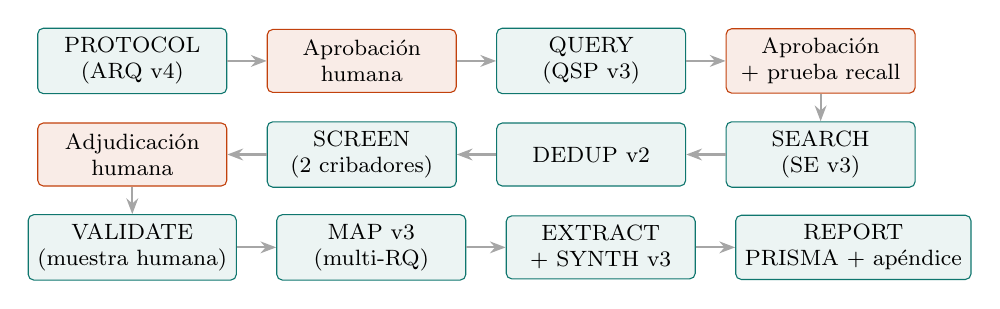
\begin{tikzpicture}[node distance=0.35cm and 0.5cm, every node/.style={font=\footnotesize},
  box/.style={draw=palet, fill=palet!8, rounded corners=2pt, minimum width=2.4cm, minimum height=0.8cm, align=center},
  hum/.style={draw=alto, fill=alto!10, rounded corners=2pt, minimum width=2.4cm, minimum height=0.8cm, align=center},
  arr/.style={-{Stealth[length=2mm]}, thick, gray!70}]
\node[box] (p) {PROTOCOL\\(ARQ v4)};
\node[hum, right=of p] (h1) {Aprobación\\humana};
\node[box, right=of h1] (q) {QUERY\\(QSP v3)};
\node[hum, right=of q] (h2) {Aprobación\\+ prueba recall};
\node[box, below=of h2] (s) {SEARCH\\(SE v3)};
\node[box, left=of s] (d) {DEDUP v2};
\node[box, left=of d] (sc) {SCREEN\\(2 cribadores)};
\node[hum, left=of sc] (h3) {Adjudicación\\humana};
\node[box, below=of h3] (v) {VALIDATE\\(muestra humana)};
\node[box, right=of v] (m) {MAP v3\\(multi-RQ)};
\node[box, right=of m] (e) {EXTRACT\\+ SYNTH v3};
\node[box, right=of e] (r) {REPORT\\PRISMA + apéndice};
\draw[arr] (p)--(h1); \draw[arr] (h1)--(q); \draw[arr] (q)--(h2); \draw[arr] (h2)--(s);
\draw[arr] (s)--(d); \draw[arr] (d)--(sc); \draw[arr] (sc)--(h3); \draw[arr] (h3)--(v);
\draw[arr] (v)--(m); \draw[arr] (m)--(e); \draw[arr] (e)--(r);
\end{tikzpicture}
\end{center}
\small Los nodos naranjas son puntos de control humano. El manifiesto de ejecución y la caché atraviesan todas las fases.\normalsize

\subsection{Estructura de directorios propuesta}
\begin{lstlisting}
palet/
  palet/                      # paquete (motor unico)
    __init__.py
    config.py                 # carga palet.toml (modelos, precios, limites)
    models.py                 # esquemas Pydantic (Apendice B)
    manifest.py               # manifiesto de ejecucion + hashes
    cache.py                  # cache content-addressed (LLM y API)
    llm.py                    # cliente Anthropic: structured outputs, retries, batches
    protocol.py               # ARQ v4
    query/                    # QSP v3: builder determinista + validadores
      builder.py  validate_scopus.py  validate_openalex.py
    sources/                  # adaptadores enchufables
      base.py  openalex.py  scopus.py  pubmed.py  citation_chasing.py
    dedup.py
    screen.py                 # SCREEN: criterio a criterio, 2 cribadores
    adjudicate.py             # export/import Excel para humanos
    validate.py               # metricas, IC, estabilidad, recall de busqueda
    mapping.py                # MAP v3
    extract.py  synthesize.py  verify_claims.py
    report/  prisma.py  checklist_prisma_scr.py  figures.py  latex.py  methods_appendix.py
    bib.py  check_citations.py
    pipeline.py               # orquestador unico (CLI y GUI lo usan)
  cli.py                      # sustituye a palet.py (mantener alias)
  app.py                      # FastAPI -> llama a palet.pipeline
  prompts/                    # versionados: screen_v1.txt, extract_v1.txt, ...
  tests/                      # pytest + fixtures grabadas (sin red)
  runs/<run_id>/              # TODO artefacto de una ejecucion vive aqui
    manifest.json protocol.yaml search_log.json records.parquet
    decisions.jsonl llm_cache/ report/
  legacy/                     # ficheros antiguos (no borrar: mover)
  palet.toml  pyproject.toml  CITATION.cff
\end{lstlisting}

% =====================================================================
\section{Paquetes de trabajo (especificación para el agente)}\label{sec:wps}

Orden recomendado: \WP{0} $\to$ \WP{1} $\to$ \WP{2} $\to$ \WP{4} $\to$ \WP{5} $\to$ \WP{6} $\to$ \WP{9} $\to$ \WP{10} (\textbf{ruta mínima para la resubmisión del capítulo}) y después \WP{3}, \WP{7}, \WP{8}, \WP{11}, \WP{12} y \WP{13}. Cada WP termina con tests en verde y una nota en \file{CHANGELOG.md}.

% ---------------------------------------------------------------
\subsection*{\WP{0} — Higiene y red de seguridad (1--2 días)}
\textbf{Objetivo}: congelar el estado actual, corregir los errores conocidos y montar los tests antes de refactorizar.
\begin{enumerate}
  \item Crear la rama \code{refactor/palet-2}. Mover a \file{legacy/} (\textbf{sin borrar}) \file{palet_legacy.py}, \file{scripts/map_module.py}, \file{scripts/report_generator.py}, \file{scripts/se_module_legacy.py} y \file{prompts/*_system.txt} sin versión.
  \item Crear \file{pyproject.toml} y \file{palet.toml}: IDs de modelo, precios por MTok, límites y \code{per_page}. Ningún ID de modelo ni precio puede quedar en el código.
  \item Corregir \code{escape_latex}: primero la barra invertida, con un mapa de un solo paso (\code{re.sub} con diccionario), y añadir un test con \verb|\ & % _ { } ~ ^ $ #| y caracteres cirílicos.
  \item Corregir \code{included} en PRISMA con un conjunto deduplicado de IDs, y añadir un test con un paper asignado a dos RQs.
  \item Eliminar la clave fantasma \code{'unmatched'} (\file{palet.py} y \file{report_generator_v2.py}) y usar \code{unmatched_not_relevant} y \code{unmatched_no_abstract}.
  \item \textbf{Errores $\neq$ exclusiones}: en MAP, cualquier fallo devuelve \code{status="error"} y la pareja (paper, RQ) se reintenta o se marca para revisión. No cuenta como ``no relevante''.
  \item Quitar el correo personal escrito en \file{se_module.py} (leerlo de \file{.env} sin valor por defecto) y cerrar el \emph{path traversal} de \code{/api/download}: resolver la ruta y exigir que esté dentro de \file{results/} o \file{runs/}.
  \item Quitar los \code{sys.exit} de los módulos de librería (lanzar excepciones) y los \code{input()} fuera de la CLI.
  \item \file{tests/} con \code{pytest}: deduplicación, \code{escape_latex}, recuentos PRISMA, parseo de OpenAlex (\emph{fixture} JSON grabada) y validación de esquemas. CI en GitHub Actions con \code{ruff} y \code{pytest}.
\end{enumerate}
\textbf{Aceptación}: \code{pytest} en verde; el \emph{pipeline} actual se ejecuta de principio a fin con \code{--max-results 10} y produce las mismas salidas que antes salvo las correcciones.

% ---------------------------------------------------------------
\subsection*{\WP{1} — Modelo de datos, manifiesto y caché (2--3 días)}
\begin{enumerate}
  \item Esquemas Pydantic (Apéndice~\ref{app:schemas}) para \code{Protocol}, \code{SearchQuery}, \code{SearchExecution}, \code{Record}, \code{ScreeningDecision}, \code{Adjudication}, \code{RQAssignment}, \code{ExtractionItem}, \code{Claim} y \code{RunManifest}.
  \item \textbf{ID estable de registro}: \code{record_id} = DOI normalizado si existe; si no, \texttt{sha1(titulo\_normalizado|primer\_autor|año)[:12]}. Prohibido usar el índice posicional. Eliminar todos los \code{iloc[paper_id]}.
  \item \code{runs/<run_id>/} como única ubicación de los artefactos de una ejecución (hoy están repartidos entre \file{outputs/json}, \file{data/raw} y \file{results}).
  \item \code{RunManifest}: \emph{hash} de git, versión de PALET, \code{model_id} exacto por fase, parámetros, \code{sha256} de cada \emph{prompt}, fecha y hora UTC de cada búsqueda, \code{meta.count} por consulta y tokens y coste reales.
  \item \code{cache.py}: clave = \code{sha256(model|system|messages|params)}. Guarda la respuesta cruda. Con \code{--replay} no se llama a ninguna API y los resultados son idénticos.
\end{enumerate}
\textbf{Aceptación}: dos ejecuciones con \code{--replay} producen \code{decisions.jsonl} idénticos byte a byte; el manifiesto contiene todos los campos.

% ---------------------------------------------------------------
\subsection*{\WP{2} — Protocolo (ARQ v4) y puntos de control (2 días)}
\begin{enumerate}
  \item Si el \emph{seed} contiene RQs, \textbf{se copian literalmente} y quedan congeladas. El LLM devuelve \code{suggested_edits} separadas, nunca sustituciones. Sin límite de 5 RQs.
  \item Criterios PCC estructurados: para cada criterio, \code{id}, \code{type} (inclusión o exclusión), \code{dimension} (population/concept/context/study\_type/language/period), \code{rule} en lenguaje operativo y \code{examples_in}/\code{examples_out}.
  \item \code{search_filters} se convierten en filtros de API reales (año, idioma, tipo) y quedan registrados.
  \item Bloques conceptuales: el LLM propone sinónimos por concepto (no una lista plana), por ejemplo \code{transition}, \code{labour}, \code{geography} y un bloque específico de cada RQ.
  \item El humano aprueba editando \file{protocol.yaml} (CLI) o un formulario (GUI). Queda registrado \code{approved_by} y \code{approved_at}.
  \item \code{temperature=0} y \code{model_id} desde la configuración.
\end{enumerate}
\textbf{Aceptación}: con el \emph{seed} ISABEL de 7 RQs se obtienen exactamente 7 RQs idénticas al texto original; el \file{protocol.yaml} pasa la validación del esquema.

% ---------------------------------------------------------------
\subsection*{\WP{3} — Búsqueda (QSP v3 + SE v3) (4--6 días)}
\begin{enumerate}
  \item \textbf{Constructor determinista}: la cadena se construye \emph{por código} a partir de los bloques conceptuales del protocolo. El LLM solo propone sinónimos. Estrategia: $Q_k = \text{TRANSICIÓN} \wedge \text{LABORAL} \wedge \text{GEO} \wedge \text{BLOQUE}_k$ para cada RQ $k$, más una consulta general sin bloque específico. Se ejecutan todas, se unen los resultados y se guarda qué consulta recuperó cada registro.
  \item \textbf{Traductores y validadores por base de datos}: OpenAlex (\code{search.title_and_abstract}, booleanos en mayúsculas, comillas en las frases) y Scopus (\code{TITLE-ABS-KEY(...)}, \code{PUBYEAR}, \code{LANGUAGE}, \code{DOCTYPE}, \code{AND NOT}, paréntesis equilibrados, $\le$ límite de longitud). Tests unitarios con cadenas válidas e inválidas.
  \item \textbf{OpenAlex}: \code{OPENALEX_API_KEY} obligatoria, cabeceras de presupuesto (\code{X-RateLimit-Remaining-USD}) registradas, \code{per_page} desde la configuración, paginación con \code{cursor=*}, reintentos con \emph{backoff} ante 429 y 5xx. Guardar \code{meta.count}, \code{relevance_score}, \code{language}, \code{type}, \code{primary_topic}, \code{topics}, países de las instituciones y \code{referenced_works}.
  \item \textbf{Sin truncado silencioso}: si \code{meta.count} supera el umbral configurado, se \emph{para} y se pide refinar o confirmar la descarga completa. Nunca se corta en silencio. Si el humano decide limitar, queda registrado y se informa.
  \item \textbf{Adaptador de Scopus} (\file{sources/scopus.py}): \code{X-ELS-APIKey} y, opcionalmente, \code{X-ELS-Insttoken}. Funciona desde la red de la Universidad de Oviedo o su VPN. Vista \code{COMPLETE} si está disponible (resúmenes); si no, recuperar los resúmenes por DOI.
  \item \textbf{Importación manual} como alternativa: aceptar CSV o RIS exportados desde la web de Scopus o WoS (el caso del capítulo). La cadena y la fecha se introducen a mano y quedan en el registro de búsqueda.
  \item \textbf{Prueba de recall de la búsqueda}: \file{protocol.yaml} admite \code{known_items} (20--40 DOIs que los autores consideran imprescindibles). Se informa del recall = encontrados / conocidos, y si es inferior a 0{,}8 se avisa y se bloquea la aprobación.
  \item (Opcional) \textbf{Búsqueda de citas} hacia atrás y hacia delante de los incluidos vía \code{referenced_works} y \code{cites:} de OpenAlex, registrada como ``otras fuentes'' en PRISMA.
  \item \code{search_log.json} con los campos de PRISMA-S: base de datos, plataforma, cadena exacta, filtros, fecha y hora, recuento total y recuento descargado.
\end{enumerate}
\textbf{Aceptación}: con el protocolo ISABEL, cada RQ tiene su consulta, los recuentos totales quedan registrados y el recall de \code{known_items} se informa.

% ---------------------------------------------------------------
\subsection*{\WP{4} — Deduplicación v2 (1 día)}
\begin{enumerate}
  \item Pasada 1: DOI normalizado (minúsculas, sin prefijo \code{https://doi.org/}, sin espacios).
  \item Pasada 2: título normalizado (minúsculas, sin acentos ni puntuación, y \textbf{partido por ``;'' o ``[''} para quedarse con la parte inglesa de los títulos bilingües) con similitud $\ge 0{,}92$ (\code{rapidfuzz.token_set_ratio}) \textbf{y} solapamiento de apellidos de autores $\ge 1$ \textbf{y} $|\Delta \text{año}| \le 1$.
  \item Los pares dudosos (similitud entre 0{,}85 y 0{,}92) se marcan para revisión humana; no se fusionan solos.
  \item Al fusionar se conserva el registro con DOI y más metadatos, y se guarda \code{merged_from}.
\end{enumerate}
\textbf{Aceptación}: test con el par Coaquira 2022 / Velásquez 2023, que debe fusionarse, y con dos falsos positivos plausibles, que no.

% ---------------------------------------------------------------
\subsection*{\WP{5} — SCREEN: cribado por criterios (4--5 días)}
\begin{enumerate}
  \item \textbf{Una llamada por registro} con salida estructurada (\emph{tool use} o esquema JSON; Apéndice~\ref{app:prompt}). Para cada criterio del protocolo: \code{met} (yes/no/unclear), \code{evidence_quote} (cita literal del título o resumen, o \code{null}) y una justificación breve.
  \item \textbf{Regla de decisión en código, no en el LLM}: incluir si se cumplen todos los criterios de inclusión y ninguno de exclusión; excluir si algún criterio es \code{no}, con \code{reason_code} igual al primero que falla según un orden fijo (Apéndice~\ref{app:reasons}); \emph{unclear} en cualquier otro caso.
  \item \textbf{Verificación de citas}: si \code{evidence_quote} no aparece en el texto (coincidencia difusa $\ge 0{,}9$), la decisión pasa a \emph{unclear}.
  \item \textbf{Dos cribadores independientes}: dos modelos distintos o el mismo con \emph{prompts} distintos, configurable. Si coinciden, la decisión es firme. Si discrepan o alguno da \emph{unclear}, pasa a adjudicación humana.
  \item \textbf{Fase de título y resumen orientada a la sensibilidad}: ante la duda, \emph{unclear}, nunca exclusión.
  \item \textbf{Adjudicación humana} (\file{adjudicate.py}): exporta a Excel los registros pendientes, con título, resumen, decisiones de A y B, citas y una columna \code{human_decision} con lista desplegable. Al reimportar se registran \code{decided_by="human:<iniciales>"} y la fecha.
  \item Registros sin resumen: intentar recuperar el resumen (Scopus por DOI u OpenAlex); si no se consigue, \code{reason_code=NO_ABSTRACT} y se informa por separado (no son ``no relevantes'').
\end{enumerate}
\textbf{Aceptación}: el 100\% de los registros tiene estado final y razón; existen las salidas \code{decisions.jsonl} y \code{screening_summary.csv}; re-cribar el corpus del capítulo (234 registros) genera razones para todas las exclusiones.

% ---------------------------------------------------------------
\subsection*{\WP{6} — VALIDATE: fiabilidad medida (2--3 días de código y 1--2 días humanos)}
\begin{enumerate}
  \item \textbf{Muestra}: todos los incluidos por PALET más una muestra aleatoria simple de los excluidos (o estratificada por razón), hasta unos 150--200 registros, con semilla fija. Se exporta a Excel \textbf{sin las decisiones de PALET} (a ciegas).
  \item \textbf{Dos humanos} (p.\,ej., Ricardo y Fernando, o un colega) criban de forma independiente con los mismos criterios. Las discrepancias se resuelven por consenso y forman el patrón de referencia.
  \item \textbf{Métricas}: sensibilidad (recall), especificidad, precisión (VPP) y F1 de PALET frente al patrón; $\kappa$ de Cohen entre humanos y entre PALET y el patrón; IC del 95\% (Wilson para proporciones, \emph{bootstrap} para $\kappa$). Si la muestra de excluidos es aleatoria, la sensibilidad se extrapola ponderando por la fracción muestreada.
  \item \textbf{Estabilidad}: re-cribar sin caché 3 veces (o con 2 modelos) un subconjunto de 100 registros e informar del porcentaje de acuerdo y de la $\kappa$ de Fleiss.
  \item Salida: \file{validation_report.json} y una tabla LaTeX lista para el capítulo.
\end{enumerate}
\textbf{Aceptación}: la tabla de validación se genera automáticamente e incluye los IC. Si la sensibilidad es inferior a 0{,}90, el informe lo marca en rojo y sugiere ajustar los criterios o el \emph{prompt}.

% ---------------------------------------------------------------
\subsection*{\WP{7} — MAP v3 (1--2 días)}
\begin{itemize}
  \item Solo se aplica a los registros \emph{incluidos}. Asignación múltiple explícita (o única, si el protocolo lo fija).
  \item Salida por pareja (registro, RQ): \code{relevance} (core/partial/none) más \code{evidence_quote}. La relevancia \code{partial} se informa por separado.
  \item Corregir el \emph{prompt}: eliminar el ejemplo~005 (inclusión con confianza baja) y la sección de ``drift''. Cada RQ incorpora su contexto, por ejemplo ``in the EU''.
\end{itemize}

% ---------------------------------------------------------------
\subsection*{\WP{8} — Extracción y síntesis anclada (4--6 días)}
\begin{enumerate}
  \item \textbf{EXTRACT} por registro incluido: lista de \code{ExtractionItem} con \code{recommendation}, \code{policy_domain} (libro de códigos configurable; para ISABEL, los seis bloques del capítulo), \code{evidence_type} (empírica, teórica, revisión o política), \code{geography}, \code{quote} literal y \code{source_text_level} (abstract o full\_text).
  \item \textbf{Texto completo opcional}: si hay versión OA (\code{best_oa_location} de OpenAlex o Unpaywall), extraer de ella y marcarlo así.
  \item \textbf{SYNTH v3}: recibe \emph{todos} los \code{ExtractionItem} de un bloque o RQ, no los 25 más citados. Devuelve frases como objetos \code{Claim}: \code{text}, \code{supporting_record_ids} (mínimo 1), \code{support_quotes} y \code{origin} (review o external).
  \item \textbf{\file{verify_claims.py}}: comprueba que cada cita aparece en el texto del registro (difusa $\ge 0{,}9$) y que la afirmación está respaldada por esa cita, mediante una segunda llamada LLM ``juez'' con salida supported/partial/unsupported. Las afirmaciones no respaldadas se eliminan o se marcan en rojo.
  \item \textbf{Mapa de evidencia}: tabla bloque $\times$ registros, con el número de estudios por bloque y por tipo de evidencia. Es justo la tabla que piden R1 y R2-M5.
  \item \textbf{Análisis de lagunas}: separar las lagunas de la literatura de los artefactos de búsqueda, por ejemplo cuando la consulta del bloque de una RQ tuvo un recuento total bajo.
\end{enumerate}
\textbf{Aceptación}: 0 afirmaciones sin IDs; al menos el 95\% de las citas verificadas; el mapa de evidencia se exporta en LaTeX y CSV.

% ---------------------------------------------------------------
\subsection*{\WP{9} — Informe, PRISMA-ScR y apéndice de métodos (3 días)}
\begin{enumerate}
  \item \textbf{Diagrama PRISMA 2020} (en inglés por defecto, idioma configurable): registros identificados por base de datos y por otras fuentes, duplicados eliminados, cribados, excluidos por razón (con desglose), no recuperables, evaluados a texto completo e incluidos. Los recuentos se calculan de \code{records} (estado final), no de \code{summary}. Exportar en PDF vectorial y en PNG a 600 ppp.
  \item \textbf{\emph{Checklist} PRISMA-ScR de 22 ítems}: cada ítem con estado \code{auto} (PALET lo rellena: fuentes, búsqueda, selección, flujo, etc.) o \code{manual} (los autores deben completarlo: protocolo y registro, evaluación crítica, etc.), con la página o sección. Nada se da por cumplido sin evidencia.
  \item \textbf{Apéndice de métodos automático} (inglés, \file{methods_appendix.tex}): modelos y versiones, fechas, cadenas exactas, filtros, criterios, número de decisiones humanas y del LLM, métricas de validación y \emph{prompts} (\emph{hash} y texto en material suplementario).
  \item \textbf{Declaración de uso de IA} alineada con RAISE: qué fases usaron IA, con qué supervisión humana, cómo se validó y cuáles son sus limitaciones.
  \item \textbf{Figuras}: etiquetas RQ (nunca ``PI''); si $n<10$ en algún grupo, gráfico de puntos con \emph{jitter} en lugar de diagrama de caja; pie con ``Citation counts: OpenAlex/Scopus, retrieved YYYY-MM-DD''; año parcial marcado; renombrar ``meta-analysis'' a ``descriptive bibliometrics''.
\end{enumerate}

% ---------------------------------------------------------------
\subsection*{\WP{10} — Bibliografía y verificador de citas del manuscrito (1--2 días)}
\begin{enumerate}
  \item Claves BibTeX estables: \texttt{ApellidoAñoPalabraTítulo} (estilo Better BibTeX), con sufijo a/b determinista. Tipo de entrada según \code{type}.
  \item \file{check_citations.py manuscrito.docx|.tex referencias.bib}: extrae las citas autor-año del texto, empareja con la lista de referencias o el \code{.bib} y produce cuatro listados: citadas y no listadas, listadas y no citadas, discrepancias de año o grafía (``Kapetaki et al.\ 2021'' frente a ``Kapetaki and Alves Dias 2021'') y duplicados a/b.
\end{enumerate}
\textbf{Aceptación}: aplicado al borrador del capítulo, reproduce al menos los casos señalados por el R2 (Green et al.\ 1997, Dijkstra et al.\ 2018, Galgóczi y Pochet 2019, la lista de no citadas, etc.).

% ---------------------------------------------------------------
\subsection*{\WP{11} — GUI y orquestación única (3--4 días)}
\begin{itemize}
  \item \file{app.py} y la CLI llaman a \code{palet.pipeline.run(...)}, que se implementa una sola vez.
  \item Puntos de control editables en la GUI: protocolo (RQs, criterios, bloques), búsqueda (cadenas y recuentos totales antes de descargar) y adjudicación (tabla con filtros, o Excel).
  \item Estado persistente por ejecución (\code{runs/<id>/state.json}) en lugar de una variable global; se puede reanudar una ejecución interrumpida.
  \item Panel de validación con métricas e IC, y panel PRISMA.
\end{itemize}

% ---------------------------------------------------------------
\subsection*{\WP{12} — Coste y rendimiento (1--2 días)}
\begin{itemize}
  \item \textbf{Message Batches API} para SCREEN, MAP y EXTRACT: más barata y sin \code{sleep}. \emph{Prompt caching} del \emph{system prompt} y del protocolo.
  \item Escalones de modelo configurables, por ejemplo: cribador A = \code{claude-sonnet-5-5}, cribador B = \code{claude-haiku-5-5}, juez y síntesis = \code{claude-opus-5-5}. Fijar siempre el ID exacto en el manifiesto y \textbf{no cambiar de modelo a mitad de una revisión}.
  \item Estimación de coste previa con los recuentos reales y un tope configurable (\code{max_cost_eur}).
\end{itemize}

% ---------------------------------------------------------------
\subsection*{\WP{13} — Documentación, citabilidad y banco de pruebas (2--3 días)}
\begin{itemize}
  \item \file{CITATION.cff} y \emph{release} etiquetada con DOI de Zenodo, para que el capítulo cite una versión concreta (responde a ``unpublished working paper'').
  \item \file{docs/METHODS.md}: descripción metodológica con referencias, apta para pegar en artículos.
  \item \textbf{Banco de pruebas}: el corpus del capítulo, con el patrón humano de \WP{6}, se guarda como \emph{benchmark} versionado. Cada cambio de \emph{prompt} o de modelo se evalúa contra él (sensibilidad, precisión y $\kappa$) antes de usarse en producción.
  \item Medio plazo: \emph{software paper} (p.\,ej., JOSS) o artículo metodológico con la validación.
\end{itemize}

% =====================================================================
\section{Plan para la revisión del capítulo}\label{sec:capitulo}

\subsection{Dos opciones para el corpus}

\begin{center}
\begin{tabularx}{\linewidth}{p{3.2cm}XX}
\toprule
 & \textbf{A. Re-cribar los 234 registros existentes} & \textbf{B. Nueva búsqueda documentada (recomendada si hay tiempo)}\\
\midrule
Qué se hace & \WP{0}+\WP{4}+\WP{5}+\WP{6}+\WP{9} sobre el CSV de Scopus importado & Lo mismo más \WP{2}+\WP{3}: búsqueda en Scopus (campus o VPN) y OpenAlex por RQ, con fecha\\
Responde a M1 & Parcialmente: la cadena original solo si se recupera del historial de Scopus. Si no, declararlo con honestidad & Totalmente: cadenas, fechas y recuentos exactos\\
Responde a M3 (RQ4 y RQ5) & No: solo puede discutir la escasez como limitación & Sí: las consultas por RQ deberían recuperar educación e inmigración\\
Coste en tiempo & 1--2 semanas & 3--4 semanas\\
Riesgo & El R2 puede insistir en la búsqueda & La Sección 4 cambia y Fernando debe re-anclar los bloques\\
\bottomrule
\end{tabularx}
\end{center}

Una vía intermedia razonable: \textbf{A más búsquedas suplementarias documentadas solo para RQ4 y RQ5}, declaradas como tales en el diagrama PRISMA (``records identified through supplementary searches''). Es una decisión de los autores.

\subsection{Pasos (opción A o intermedia)}
\begin{enumerate}
  \item \textbf{Recuperar la cadena original} de Scopus (historial de búsqueda de la cuenta, correo de exportación o notas de mayo de 2025). Si no aparece, decirlo.
  \item Importar \file{Final_Fernando_3.1.csv} (235 registros), localizar el registro perdido y deduplicar con \WP{4}. Resultado esperado: 1 duplicado (Perú).
  \item Fijar los criterios PCC con Fernando (propuesta en el Apéndice~\ref{app:protocol}).
  \item Re-cribar con \WP{5}, adjudicar con \WP{5}.6 y validar con \WP{6} (Ricardo y Fernando a ciegas).
  \item Re-asignar las RQs con \WP{7}, aplicar extracción y mapa de evidencia con \WP{8} y entregar el mapa a Fernando para revisar M4 y M5 cita por cita.
  \item Generar el diagrama PRISMA, el \emph{checklist}, el apéndice y las figuras con \WP{9}. Ejecutar \file{check_citations.py} sobre el manuscrito.
\end{enumerate}

\subsection{Plantillas de texto para el capítulo (inglés; completar tras la re-ejecución)}

\begin{nota}[Methods (reproducibility paragraph) — borrador]
\small
\emph{The search was run in Scopus (title, abstract and keywords) on [DATE] using the search string reported in Appendix~A ([N\_ID] records), restricted to [YEARS], [LANGUAGES] and [DOCUMENT TYPES]. PALET v[X.Y] (Zenodo DOI [..]) was used for de-duplication, title-and-abstract screening and question mapping, with Anthropic Claude models ([EXACT MODEL IDs]) called through the API at temperature 0. Each record was assessed against pre-specified eligibility criteria (Appendix~B) by two independent model configurations; disagreements and uncertain cases ([N\_H] records) were adjudicated by the authors. Screening and extraction were based on [titles and abstracts / open-access full texts]. The PRISMA-ScR flow diagram and checklist are provided in Figure~[X] and Supplementary Material~[Y].}
\end{nota}

\begin{nota}[Validation and limitations — borrador]
\small
\emph{To assess the reliability of the AI-assisted screening, two authors independently and blindly screened a random sample of [N] records (all [n\_inc] included and [n\_exc] excluded records). Against the consensus human decision, PALET achieved a sensitivity of [..] (95\% CI [..]), a precision of [..] (95\% CI [..]) and Cohen's $\kappa$ of [..]. Repeated runs agreed in [..]\% of decisions. The procedure is AI-assisted rather than objective: it may miss relevant studies (especially those not indexed in the searched database or described with different terminology), its outputs depend on the model version, and screening on abstracts may misclassify studies whose relevance is only apparent in the full text. Evidence for [RQ4 and RQ5] is thin ([n] and [n] studies), and conclusions for these blocks should be read as indicative.}
\end{nota}

\textbf{Frases que hay que retirar del capítulo}: ``objective'', ``ensures a complete sweep of key references'', ``fully automated'', ``brief meta-analysis'' y toda descripción de pasos que no se ejecutaron (filtrado PRISMA o síntesis contextualizada en la versión de 2025).

\textbf{Respuesta a la parte de agentes (R1)}: reducir Wooldridge y Jennings, Shoham y Green et al.\ a un párrafo, como pide el R2, y añadir referencias recientes de agentes basados en LLM (p.\,ej., Yao et al., ReAct, ICLR 2023; Wang et al., ``A survey on large language model based autonomous agents'', \emph{Frontiers of Computer Science}, 2024). Comprobar las referencias exactas antes de citarlas. En cuanto a Chain-of-Thought, quitar la nota al pie y dejar solo la cita, y revisar el año de Wei et al.\ (NeurIPS 2022).

% =====================================================================
\section{Qué significa ``una herramienta de 10''}

\begin{center}
\begin{tabularx}{\linewidth}{Xl}
\toprule
\textbf{Criterio verificable} & \textbf{Umbral}\\
\midrule
Recall de la búsqueda frente a \code{known_items} & $\ge 0{,}90$\\
Sensibilidad del cribado de título y resumen frente al patrón humano & $\ge 0{,}95$ (IC informado)\\
Precisión del cribado & $\ge 0{,}50$ (informada siempre)\\
$\kappa$ PALET--patrón humano & $\ge 0{,}70$ (informada siempre)\\
Registros con estado final y razón & 100\%\\
Afirmaciones de síntesis con IDs y cita verificada & 100\% con IDs y $\ge 95\%$ verificadas\\
Re-ejecución con \code{--replay} & idéntica byte a byte\\
\emph{Checklist} PRISMA-ScR & 22/22 ítems con estado y ubicación\\
Cobertura de tests del paquete \file{palet/} & $\ge 70\%$; CI en verde\\
IDs de modelo, \emph{prompts} y fechas en el manifiesto & 100\%\\
Versión citable (DOI) & sí\\
\bottomrule
\end{tabularx}
\end{center}

La literatura reciente sobre cribado con LLM muestra un rendimiento muy variable entre revisiones y advierte de que todavía no se recomienda automatizar por completo el cribado de título y resumen. La sensibilidad es la métrica crítica. Por eso el diseño propuesto no promete automatización total: \textbf{promete una asistencia medida, con un humano responsable}, que es lo que exigen la declaración conjunta Cochrane/Campbell/JBI/CEE y RAISE.

% =====================================================================
\section{Instrucciones operativas para el agente implementador}\label{sec:instrucciones}

\begin{agente}[Reglas de trabajo]
\begin{enumerate}[leftmargin=*]
  \item \textbf{Idioma}: habla con Ricardo en español. El código, los identificadores, los \emph{docstrings} y los mensajes de \emph{commit} van en inglés. Los textos de interfaz pueden seguir en español.
  \item \textbf{Ritmo}: Ricardo trabaja de forma secuencial y quirúrgica. Haz \textbf{un WP cada vez}; dentro de cada WP, un fichero o cambio coherente cada vez. Al final de cada paso, da un resumen breve (qué cambió, por qué y cómo probarlo) con el comando exacto que debe ejecutar, y espera su confirmación (suele responder ``continuar'').
  \item \textbf{Entorno}: macOS en Apple Silicon, Python 3.12 de Homebrew (nativo arm64), VS Code y MacTeX. Usa un único entorno virtual \file{.venv} y no toques \file{venv/} ni \file{palet_env/}: propón eliminarlos y deja que Ricardo decida.
  \item \textbf{No borres nada}: mueve a \file{legacy/}. No modifiques \file{results/}, \file{outputs/} ni \file{data/raw/} históricos; escribe todo lo nuevo en \file{runs/}.
  \item \textbf{Secretos}: nunca escribas claves ni correos en el código. Variables nuevas en \file{.env.example}: \code{OPENALEX_API_KEY}, \code{ELSEVIER_API_KEY}, \code{ELSEVIER_INSTTOKEN} (opcional) y \code{CONTACT_EMAIL}.
  \item \textbf{Coste}: antes de cualquier ejecución real con LLM de más de 1\,€ (estimado), muestra la estimación y pide permiso. En desarrollo usa \code{--max-records 20} y la caché.
  \item \textbf{Tests primero} en las correcciones de errores: escribe el test que falla, corrige y comprueba que pasa.
  \item \textbf{Compatibilidad}: mantén \code{python palet.py --seed-prompt ...} como alias de la nueva CLI hasta terminar \WP{11}.
  \item \textbf{Verifica antes de afirmar}: este informe cita líneas y ficheros de la versión \code{da90731}. Si algo no coincide, dilo y no supongas.
  \item \textbf{Decisiones de método} (criterios PCC, opción A o B, umbrales, asignación única o múltiple): son de Ricardo y Fernando. Propón, no decidas.
\end{enumerate}
\end{agente}

% =====================================================================
\appendix

\section{Lista de errores con ubicación}\label{app:bugs}
\small
\begin{longtable}{p{0.7cm}p{4.6cm}p{9.6cm}}
\toprule
\textbf{Sev.} & \textbf{Ubicación} & \textbf{Problema y solución}\\
\midrule
\endhead
\sevC & \file{prisma_validator.py}, \code{build_prisma_data} & \code{included} suma longitudes por RQ $\to$ usar \code{len(set().union(*rq_lists))}\\
\sevC & \file{map_module_v2.py}, \code{analyze_paper} (ramas de error) & El error devuelve \code{assignments: []} y cuenta como ``no relevante'' $\to$ \code{status="error"}\\
\sevC & \file{se_module.py}, \code{search_openalex} & \code{search} incluye el texto completo; sin \code{api_key}; truncado sin \code{meta.count}\\
\sevC & \file{arq_module.py} y \file{arq_system_v3.txt} & Reescribe y limita las RQs a 1--5\\
\sevA & \file{report_generator_v2.py:46} & Orden de \code{escape_latex} (barra invertida al final)\\
\sevA & \file{report_generator_v2.py:885, 1082}; \file{palet.py} (resumen) & Clave fantasma \code{'unmatched'}\\
\sevA & \file{report_generator_v2.py:141, 1026, 1094}; \file{synthesis_module.py} & \code{iloc[int(paper_id)]} posicional $\to$ \code{record_id}\\
\sevA & \file{se_module.py}, \code{remove_duplicates} & Solo DOI exacto o título exacto\\
\sevA & \file{qsp_module.py}, \code{suggest_query_structure} & Esquema contradictorio con el \emph{system prompt}; \code{json.loads} sin limpieza robusta; sin validación\\
\sevA & \file{app.py}, \code{/api/download} & \emph{Path traversal}\\
\sevA & \file{app.py} y \file{palet.py} & Orquestación duplicada\\
\sevA & \file{export_bibtex.py} & Claves inestables; todo como \code{@article}\\
\sevM & \file{se_module.py:20} & Correo personal como valor por defecto en un repositorio público\\
\sevM & Varios (5 ficheros) & \code{model=} escrito a mano; \file{map_module.py} con \code{claude-sonnet-4-20250514}\\
\sevM & \file{arq_module.py}, \code{qsp_module.py} & Sin \code{temperature}; \code{sys.exit} al importar\\
\sevM & \file{map_system_v2.txt} & Ejemplo 005 (incluye con confianza baja); sección ``drift''\\
\sevM & \file{synthesis_module.py} & Top 25 por citas; resúmenes truncados a 1.200 caracteres; sin citas por afirmación\\
\sevB & \file{README.md} & \code{YOUR_USERNAME}; afirmación ``reproducibility'' con \code{temperature=0}\\
\bottomrule
\end{longtable}
\normalsize

\section{Esquemas de datos (Pydantic v2)}\label{app:schemas}
\begin{lstlisting}[language=Python]
from datetime import datetime
from typing import Literal, Optional
from pydantic import BaseModel, Field

Dimension = Literal["population", "concept", "context",
                    "study_type", "language", "period"]

class Criterion(BaseModel):
    id: str                      # "IC1", "EC3"
    kind: Literal["include", "exclude"]
    dimension: Dimension
    rule: str                    # operational wording
    examples_in: list[str] = []
    examples_out: list[str] = []

class ConceptBlock(BaseModel):
    name: str                    # "transition", "labour", "geo", "rq4_education"
    terms: list[str]
    applies_to_rqs: list[str] = []   # [] = all

class Protocol(BaseModel):
    version: int
    title: str
    research_questions: dict[str, str]          # {"RQ1": "...", ...} frozen
    criteria: list[Criterion]
    concept_blocks: list[ConceptBlock]
    sources: list[Literal["scopus", "openalex", "pubmed", "wos", "manual_import"]]
    year_from: Optional[int] = None
    year_to: Optional[int] = None
    languages: list[str] = ["en"]
    document_types: list[str] = ["article", "review"]
    known_items: list[str] = []                 # DOIs for search-recall test
    assignment_mode: Literal["single", "multi"] = "multi"
    approved_by: Optional[str] = None
    approved_at: Optional[datetime] = None

class SearchExecution(BaseModel):
    query_id: str                # "Q_RQ4_scopus"
    source: str
    platform: str                # "Scopus Search API", "OpenAlex API", "Scopus web export"
    query_string: str
    filters: dict
    executed_at: datetime
    total_hits: int              # meta.count / opensearch:totalResults
    downloaded: int
    truncated: bool
    truncation_approved_by: Optional[str] = None

class Record(BaseModel):
    record_id: str               # DOI or sha1(title|first_author|year)[:12]
    doi: Optional[str]
    title: str
    abstract: Optional[str]
    authors: list[str]
    year: Optional[int]
    source_title: Optional[str]
    language: Optional[str]
    doc_type: Optional[str]
    affiliation_countries: list[str] = []
    found_by_queries: list[str]
    merged_from: list[str] = []
    status: Literal["identified", "duplicate", "ta_included", "ta_excluded",
                    "ta_unclear", "ft_excluded", "included", "error"]

class CriterionJudgement(BaseModel):
    criterion_id: str
    met: Literal["yes", "no", "unclear"]
    evidence_quote: Optional[str]
    quote_verified: bool = False
    rationale: str = Field(max_length=300)

class ScreeningDecision(BaseModel):
    record_id: str
    screener: str                # "llm_a:claude-sonnet-5-5" | "human:RMVP"
    judgements: list[CriterionJudgement]
    decision: Literal["include", "exclude", "unclear", "error"]
    reason_code: Optional[str]   # see reason codes appendix
    prompt_sha256: str
    decided_at: datetime

class ExtractionItem(BaseModel):
    record_id: str
    recommendation: str
    policy_domain: str           # codebook value
    evidence_type: Literal["empirical", "theoretical", "review", "policy_document"]
    geography: list[str]
    quote: str
    quote_verified: bool
    source_text_level: Literal["abstract", "full_text"]

class Claim(BaseModel):
    text: str
    supporting_record_ids: list[str] = Field(min_length=1)
    support_quotes: list[str]
    origin: Literal["review", "external"]
    verdict: Optional[Literal["supported", "partial", "unsupported"]] = None
\end{lstlisting}

\section{Esqueleto del \emph{prompt} de cribado}\label{app:prompt}
\begin{lstlisting}
<role>You screen records for a scoping review. You do NOT decide inclusion;
you judge each eligibility criterion separately. Code applies the decision rule.</role>

<protocol>
Review title: {title}
Research questions (context only, do not screen on them): {rqs}
Criteria:
{for each criterion: id | include/exclude | dimension | rule | examples_in | examples_out}
</protocol>

<instructions>
1. Read ONLY the title and abstract given. Do not use outside knowledge about the paper.
2. For EVERY criterion return met = yes | no | unclear.
   - "yes"/"no" REQUIRE an evidence_quote copied verbatim from title/abstract.
   - If the text does not let you decide, answer "unclear" (never guess "no").
3. Geography: a study is in scope only if its empirical or policy focus includes
   the EU/EU member states (as defined in the protocol). Global studies count only
   if they report EU-specific results.
4. Keep rationale <= 40 words.
</instructions>

<output> Call the tool `record_screening` with the JSON schema provided. </output>
\end{lstlisting}

\section{Códigos de razón de exclusión (orden de precedencia)}\label{app:reasons}
\begin{center}
\small
\begin{tabularx}{\linewidth}{lX>{\raggedright\arraybackslash}p{3.6cm}}
\toprule
\textbf{Código} & \textbf{Significado} & \textbf{Ejemplo en el corpus}\\
\midrule
\code{DUPLICATE} & Duplicado fusionado & Velásquez 2023 / Coaquira 2022\\
\code{WRONG_DOC_TYPE} & Tipo de documento fuera del protocolo & editorial, nota\\
\code{WRONG_LANGUAGE} & Idioma fuera del protocolo & —\\
\code{OUT_OF_PERIOD} & Fuera del periodo & —\\
\code{WRONG_CONTEXT} & Fuera del ámbito geográfico (no UE) & Ye et al.\ 2014 (China)\\
\code{WRONG_CONCEPT} & Sin dimensión de empleo o mercado laboral & Jedelhauser y Binder 2015\\
\code{WRONG_PHENOMENON} & Sin vínculo con la transición verde o digital & Pobedin 2024\\
\code{NO_POLICY_CONTENT} & Sin recomendaciones ni análisis de política (si el protocolo lo exige) & —\\
\code{NO_ABSTRACT} & Sin resumen recuperable (se informa aparte) & —\\
\bottomrule
\end{tabularx}
\end{center}

\clearpage
\section{Propuesta de protocolo para el capítulo ISABEL (a validar por los autores)}\label{app:protocol}
\begin{lstlisting}
version: 1
title: "Policies for job creation and destruction linked to the EU twin transition"
research_questions:            # copied verbatim from Table 2 of the chapter
  RQ1: "What economic-policy recommendations does the literature formulate to mitigate job destruction and boost job creation associated with the green transition in the EU?"
  RQ2: "What recommendations does the literature provide regarding the impact of digitalisation and artificial intelligence on JCD in the EU?"
  RQ3: "What cohesion or smart-specialisation policies does the evidence suggest?"   # consider adding: "to address JCD from the twin transition in EU regions"
  RQ4: "Which initial-education and lifelong-learning models are most effective for adapting green and digital skills?"
  RQ5: "What role do immigration and labour mobility play in filling skill gaps during the transition?"
  RQ6: "How should just-transition policies be designed to prevent green and digital discontent in territories that depend on fossil fuels or have low levels of digitalisation?"
  RQ7: "What knowledge gaps persist regarding the measurement and forecasting of JCD and the effectiveness of the cited policies?"
assignment_mode: multi
criteria:
  - {id: IC1, kind: include, dimension: context,
     rule: "Empirical or policy focus on the EU, EU member states or their regions (UK pre-2020 allowed: DECIDE)"}
  - {id: IC2, kind: include, dimension: concept,
     rule: "Addresses employment, jobs, skills, labour markets or labour mobility"}
  - {id: IC3, kind: include, dimension: concept,
     rule: "Linked to the green and/or digital transition (decarbonisation, energy transition, automation, AI, digitalisation)"}
  - {id: IC4, kind: include, dimension: study_type,
     rule: "Peer-reviewed article or review"}
  - {id: EC1, kind: exclude, dimension: context,
     rule: "Exclusively non-European setting without EU-specific results"}
  - {id: EC2, kind: exclude, dimension: concept,
     rule: "Purely environmental/technical analysis without labour-market or policy dimension"}
year_from: 2013
year_to: 2025
languages: [en, es]
document_types: [article, review]
sources: [scopus, openalex]     # or: [manual_import] for option A
known_items: []                 # FILL: 20-40 DOIs the authors consider essential
\end{lstlisting}

% =====================================================================
\section{Referencias y fuentes externas}\label{sec:refs}
\small
\begin{itemize}
  \item Tricco, A.\,C. et al.\ (2018). PRISMA Extension for Scoping Reviews (PRISMA-ScR): checklist and explanation. \emph{Annals of Internal Medicine}, 169(7), 467--473. doi:10.7326/M18-0850.
  \item Page, M.\,J. et al.\ (2021). The PRISMA 2020 statement. \emph{BMJ}, 372, n71. doi:10.1136/bmj.n71.
  \item Rethlefsen, M.\,L. et al.\ (2021). PRISMA-S: an extension to the PRISMA statement for reporting literature searches in systematic reviews. \emph{Systematic Reviews}, 10, 39. doi:10.1186/s13643-020-01542-z.
  \item Peters, M.\,D.\,J. et al.\ (2020). Updated methodological guidance for the conduct of scoping reviews. \emph{JBI Evidence Synthesis}, 18(10), 2119--2126. doi:10.11124/JBIES-20-00167.
  \item Flemyng, E. et al.\ (2025). Position statement on artificial intelligence (AI) use in evidence synthesis across Cochrane, the Campbell Collaboration, JBI and the Collaboration for Environmental Evidence 2025. \emph{Campbell Systematic Reviews}, 21, e70074. doi:10.1002/cl2.70074. Se apoya en las recomendaciones RAISE.
  \item Huotala, A., Kuutila, M. y Mäntylä, M. (2025). SESR-Eval: Dataset for evaluating LLMs in the title-abstract screening of systematic reviews. arXiv:2507.19027.
  \item Haddaway, N.\,R. et al.\ (2022). PRISMA2020: An R package and Shiny app for producing PRISMA 2020-compliant flow diagrams. \emph{Campbell Systematic Reviews}, 18, e1230. doi:10.1002/cl2.1230.
  \item OpenAlex: documentación de búsqueda (\url{https://help.openalex.org/api/searching}) y de autenticación y precios (\url{https://developers.openalex.org/api-reference/authentication}). Consultadas el 11/11/2026.
  \item Elsevier Developer Portal: Scopus Search API y autenticación por IP o \emph{InstToken} (\url{https://dev.elsevier.com}). Consultado el 11/11/2026.
\end{itemize}

\end{document}
